\chapter{Design measurements}
\label{cha:measurements}
For measuring different simulation designs a example network was implemented using a monolithic and a modular design.
These implementations represent examples of the designs discussed in chapter \ref{cha:design}.
The simulation of this network using the different designs is used for analyzing the impact on the performance.


\section{Simulated example network}
\label{sec:measurements_network}
The example network simulates a message queue with different types of transmitted data (configuration, event, historical).
The different types of data are processed by different parts within the network.
This network includes parts for data generation and data processing.
Such a exemplary network was chosen, due to multiple similar practical applications.
An overview of the simulated network is shown in Figure \ref{fig:design_test_network}.

\begin{figure}
    \centering
    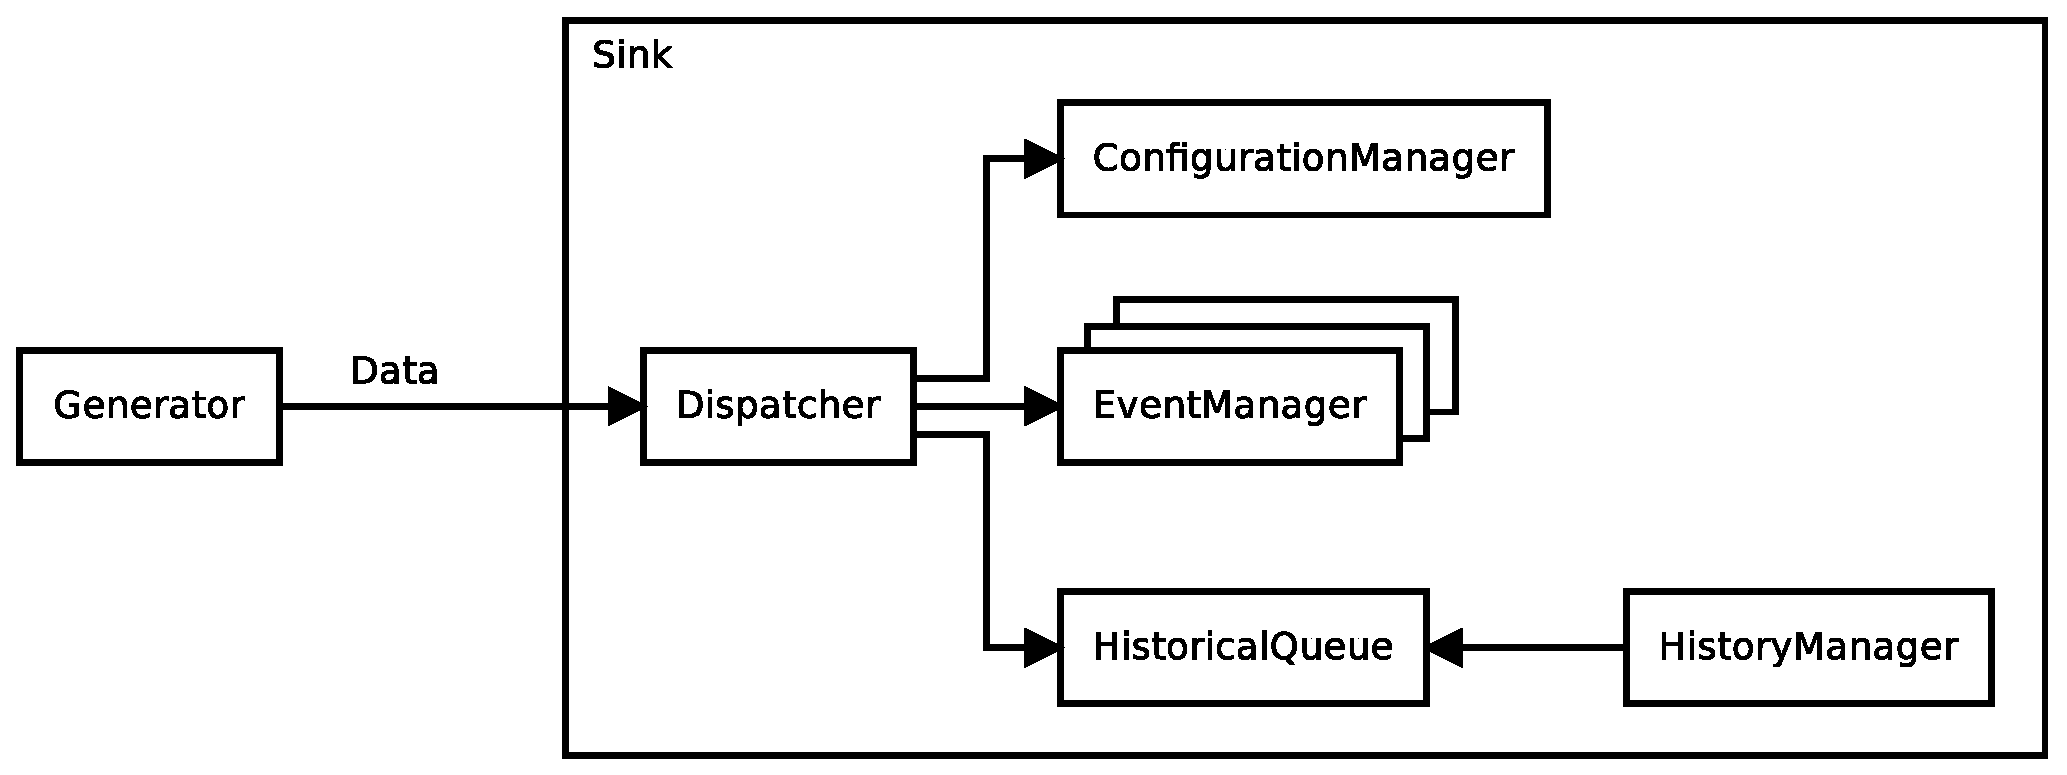
\includegraphics[width=0.9\linewidth]{design_test_network.eps}
    \caption{Example network including generator, sink, queue and different manager.}
    \label{fig:design_test_network}
\end{figure}

The \emph{Generator} generates cyclic data and a polling command.
Both are transmitted via messages to the sink module.
The generated data includes a field of 64 Bytes and a enumeration describing the type of data.
The generated polling command triggers the polling of the \emph{HistoryManager}.

These messages are transmitted to a sink, which is described via the interface module \emph{ISink}.
The differently designed modules \emph{ModularSink} and \emph{MonolithicSink} extend the interface and represent the different tested designs.

The first part within the sink is the \emph{Dispatcher} which is accessing the type information of the data and then forwards the packed data to the according parts.
Configuration and are forwarded to the \emph{ConfigurationManager} whereas the event data are forwarded to the \emph{EventManagers}.
The simulated network provides a variable number of eventmanagers and all generated event data are dispatched to the eventmanagers sequentially.
The \emph{ConfigurationManager} and the \emph{EventManagers} are simple implementations which executes various calculations on the received data to simulate processing.
Historical data are forwarded to the \emph{HistoricalQueue} which is internally implemented by a std::queue which holds all received data until they are accessed.
The \emph{HistoryManager} accesses the \emph{HistoricalQueue} and processes available data similar to \emph{ConfigurationManager} and \emph{EventManager} by executing dummy calculations.
This access is initiated by a configurable polling interval.
\\

The functionality of dispatching and processing of the data is, as shown in Figure \ref{fig:design_test_network}, is included in the sink and is implemented twice with different designs.

The assumption of existing implementations for the \emph{Dispatcher}, \emph{ConfigurationManager}, \emph{EventManager} and \emph{HistoryManager} which must not be changed for the simulation is made.
Therefore implementing the \emph{MonolithicSink} consists of instantiating and connecting the different parts within a single simple module.
Received messages will be analyzed and the enclosed data is forwarded to the according instances.
The polling done by the \emph{ConfigurationManager} is implemented using \emph{self-messages} sent in an configurable interval.

Implementing the \emph{ModularSink} requires the implementation of wrapper modules for every single part which should be represented by a separate module.
These wrapper extract the transmitted data of received messages and forward it to the enclosing parts.
Calls from within the enclosed parts are handled by methods of the wrappers, which are passed via function pointers (functional objects).
Within this methods according messages are created and sent via output gates.
The internal structure of the \emph{ModularSink} is shown in figure \ref{fig:ModularSink}.
Within the \emph{ModularSink} arrays of gates, connections and \emph{EventWrapper} are used for realizing a variable number of \emph{EventManagers}.

\begin{figure}
    \centering
    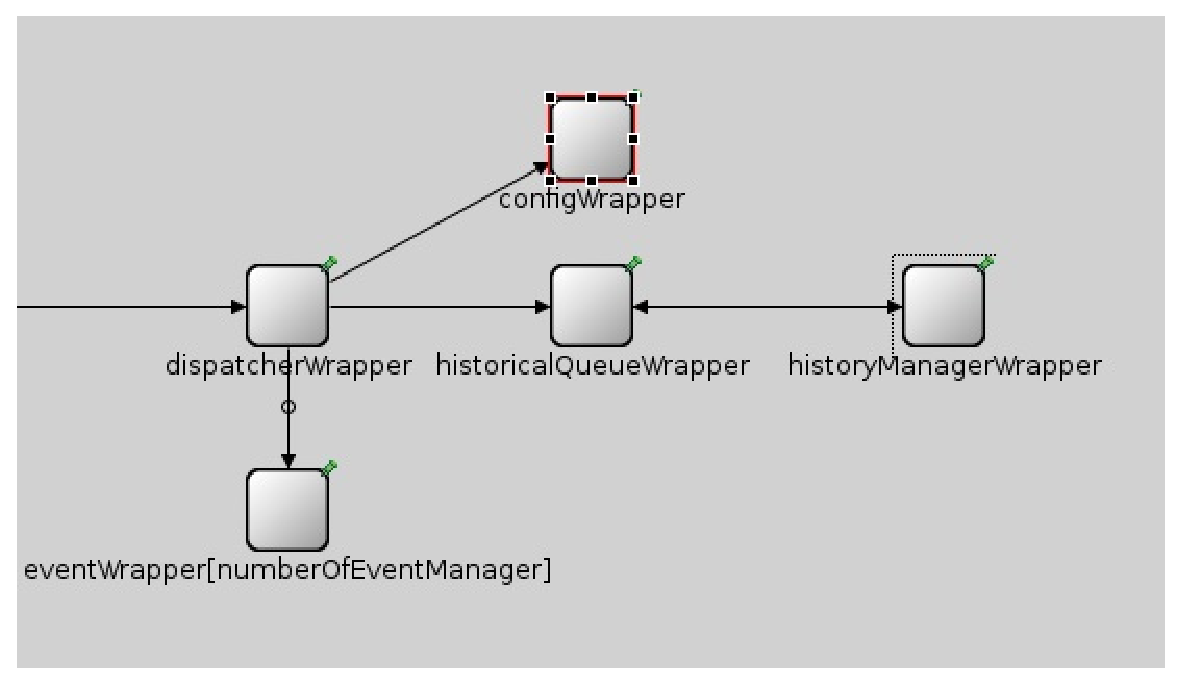
\includegraphics[width=0.9\linewidth]{images/ModularSink}
    \caption{Structure of \emph{ModularSink} showing the implemented Wrapper modules and their connections.}
    \label{fig:ModularSink}
\end{figure}

The simulated network is shown in figure \ref{fig:omnet_example_network}.

\begin{figure}
    \centering
    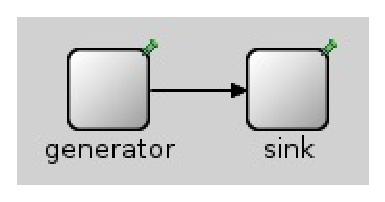
\includegraphics[width=0.3\linewidth]{images/omnet_example_network}
    \caption{Simulated example network showing the \emph{Generator} instance and its connection to the instance of the sink module derived from \emph{ISink}.}
    \label{fig:omnet_example_network}
\end{figure}

\section{Measurement methods}
\label{sec:measurements_methods}
For measuring the performance of the different designs three measurement methods were implemented.
These methods were implemented via different scripts for automated executing and designed dynamically allowing the analyze of various simulations and also either sequential or parallel simulation.

\subsection{Runtime measurement}
\label{sec:measurements_methods_runtime}
The performance of the simulated design can be analyzed by defining a fixed simulation time limit (\emph{sim-time-limit}).
Using the default (non real-time) scheduler this results in a simulation which executes as fast as possible for the needed number of event for reaching the simulation time limit.
The required time for this simulation represents the performance of the simulation.

Analyzing a parallel simulation using this method does not require special attention, except the handling of multiple resulting runtime values.

\subsection{Processed event count}
\label{sec:measurements_methods_event}
By defining a fixed execution time limit (\emph{cpu-time-limit}) and using the default scheduler the simulation will run for a fixed time.
The number of processed events within this fixed time represents the performance of the simulation.

The simulation of different designs results in contrasting event counts due to the increased number of messages within a modular design.
Therefore for evaluating the created number within a fixed processing time the ratio of event creation must be determined.
This ratio can be measured using the previous method \ref{sec:measurements_methods_runtime}.

\subsection{Real time behavior}
\label{sec:measurements_methods_realtime}
Using the built in real time scheduler \emph{cRealTimeScheduler} the simulation will try to execute the simulation matching the real time.
The performance output (\emph{cmdenv-performance-display}) provides the ratio of simulated seconds per real second.
As described in section \ref{sec:simulation_omnet} this ratio must not differ too much from one for representing a real-time simulation.
The simulated network provides a configurable interval of data/command generation.
Using a parameter study (described in section \ref{sec:omnet_running_config}) the interval for data/command generation can be set with values form a range of intervals.
With attention to the performance ratio of the different iterations the interval limit, which still allows real-time simulation, can be determined.

\subsection{Result recording}
The results of the different measurement methods are all extracted from the resulting command line output of the simulation.
The automated test scripts are analyzing the outputs of the executed simulation after finishing the simulation.
For preventing the delay of the measurements and the simulation by writing the output to a file located on an slow peripheral the output files are located on a \emph{ramdisk}.
A \emph{ramdisk} represents a filesystem which is located within the \emph{RAM} (Random access memory) and therefore provides the maximum speed for writing and analyzing outputs.

The implemented test network described in \ref{sec:measurements_network} was developed and analyzed on a Lenovo ideapad U530 with 8GB PC3-12800 DDR3 SDRAM 1600 MHz and a 4th Gen Intel® Core™ i7-4500U (1.8 GHz 200 MHz 4MB) running Kubuntu 15.10.
\cite{lenovo_spec}\\

%TODO: find correct place for specs and add APC spec and execute simulation on APC


\section{Sequential Simulation}
\label{sec:measurements_sequential}
Each of the three developed measurement methods was executed multiple times with the example network.
To eliminate a possible dependency of the resulting performance to the simulated range (e.g. period of simulation time) each method was executed with different times.
The runtime and real-time method was executed for multiple values for the simulation time limit and the event method was executed for different cpu time limits.
This variation of simulation time also verifies the testing measurements for independence of the simulated time range.

For multiple load scenarios three parameter studies (parameter sweeps) were executed for each testing method.

\begin{itemize}
    \item Number of EventManager
    \item Generation interval of \emph{Generator}
    \item Polling interval of \emph{HistoryManager}
\end{itemize}

In the following section the measurement result of the evaluation test (sweep of simulation or cpu time) and the results of the load tests are shown and analyzed.

\subsection{Runtime}
\label{sec:measurements_sequential_runtime}

The runtime results of the sequential simulations using both designs and given different simulation time limits are displayed in figure \ref{fig:results_runtime_sim_time}.
The double logarithmic axis shows two linear plots for modular and monolithic design.
These nearly parallel linear plots show a constant factor in between the runtimes using the two different designs.
The average ratio of runtime using the modular design over the runtime using the monolithic design is 9999. %TODO refresh
\\

%TODO check if necessary
% \[\frac{\sum\frac{t_{modular}}{t_{monolithic}}}{N} = 2.84\]

%%% runtime over simulation time %%%
\begin{figure}
    \centering
    \pgfplotsset{
        every axis plot/.append style={very thick}
    }
    \begin{tikzpicture}
        \begin{axis}[
        xmode=log,
        ymode=log,
        ylabel={Runtime $[s]$},
        xlabel={Simulation time $[s]$},
        grid=major,
        legend entries={Modular,Monolithic},
        legend style={at={(0,1)}, anchor=north west}
        ]
        
        \addplot table {results/runtimeResults.Modular.txt};
        \addplot table {results/runtimeResults.Monolithic.txt};
        \end{axis}
    \end{tikzpicture}    
    \caption{Runtime using different designs over different simulation time limits.}
    \label{fig:results_runtime_sim_time}
\end{figure}

The following measurement were made with a fixed simulation time limit of 1 minute.

The runtime using different designs with a varying number of \emph{EventManagers} is shown in figure \ref{fig:results_runtime_eventmanager}.
\\
%TODO explain

%%% runtime over number of event manager %%%
\begin{figure}
    \centering
    \pgfplotsset{
        every axis plot/.append style={very thick}
    }
    \begin{tikzpicture}
    \begin{axis}[
    %xmode=log,
    %ymode=log,
    ylabel={Runtime [s]},
    xlabel={Number of \emph{EventManager}},
    grid=major,
    legend entries={Modular,Monolithic},
    legend style={at={(0,1)}, anchor=north west}
    ]
    
    \addplot table {results/time/simtimeEventManagerResults.Modular.txt};
    \addplot table {results/time/simtimeEventManagerResults.Monolithic.txt};
    \end{axis}
    \end{tikzpicture}    
    \caption{Runtime using different designs over variing number of \emph{EventManager}.}
    \label{fig:results_runtime_eventmanager}
\end{figure}

The runtime using different designs with a varying polling interval of \emph{HistoryManager} is shown in figure \ref{fig:results_runtime_polling}.
These results are again shown in a double logarithmic plot for easier recognition of both plots following a potential characteristic of sinking required runtime with increasing polling interval.
The offset in between the two plots shown in figure \ref{fig:results_runtime_polling} is due to the double logarithmic display representing the ratio in between the runtimes using different designs.
The average ratio of runtime using the modular design over the runtime using the monolithic design is $7.844$.
\\
%%% runtime over polling interval %%%
\begin{figure}
    \centering
    \pgfplotsset{
        every axis plot/.append style={very thick}
    }
    \begin{tikzpicture}
    \begin{axis}[
    xmode=log,
    ymode=log,
    ylabel={Runtime [s]},
    xlabel={Polling interval [ns]},
    grid=major,
    legend entries={Modular,Monolithic},
    legend style={at={(1,1)}, anchor=north east}
    ]
    
    \addplot table {results/time/simtimePollingResults.Modular.txt};
    \addplot table {results/time/simtimePollingResults.Monolithic.txt};
    \end{axis}
    \end{tikzpicture}    
    \caption{Runtime using different designs over varying polling interval by \emph{HistoryManager}.}
    \label{fig:results_runtime_polling}
\end{figure}

The runtime using different designs with a varying generation interval of \emph{Generator} is shown in figure \ref{fig:results_runtime_generation}.
Similar to the previous figure these results are also shown in a double logarithmic plot showing the potential characteristic of sinking required runtime with increasing generation interval.
Again the noticeable offset in between the plots is due to a ratio of resulting runtimes.
The average ratio of runtime using the modular design over the runtime using the monolithic design is $1.758$.
\\

%%% runtime over generation interval %%%
\begin{figure}
    \centering
    \pgfplotsset{
        every axis plot/.append style={very thick}
    }
    \begin{tikzpicture}
    \begin{axis}[
    xmode=log,
    ymode=log,
    ylabel={Runtime [s]},
    xlabel={Generation interval [ns]},
    grid=major,
    legend entries={Modular,Monolithic},
    legend style={at={(1,1)}, anchor=north east}
    ]
    
    \addplot table {results/time/simtimeGenerationResults.Modular.txt};
    \addplot table {results/time/simtimeGenerationResults.Monolithic.txt};
    \end{axis}
    \end{tikzpicture}    
    \caption{Runtime using different designs over varying generation interval by \emph{Generator}.}
    \label{fig:results_runtime_generation}
\end{figure}


Analyzing the resulting outputs the ratio of generated messages (events) regarding the different designs can be determined.
The average ratio of number of created events using the modular design over the number of created events using the monolithic design is $2.143$.%TODO refresh
This ratio will be used as correction value for the next measurement method analyzing the created events within a fixed cpu time.

\subsection{Created events}
\label{sec:measurements_sequential_event}

The results testing the simulations and analyzing the number of created events within a given cpu time are displayed in figure \ref{fig:results_event_cpu_time}.
Similar to the runtime results a double logarithmic display was used for analyzing the characteristic of the plots.
The courses show potential characteristics and are nearly linear and parallel this leads to the assumption of a constant ratio in between the used designs.
The average ratio of number of created events using the modular design over the number of created event using the monolithic design is 9999. %TODO refresh
\\

%%% event number over cpu time %%%
\begin{figure}
    \centering
    \pgfplotsset{
        every axis plot/.append style={very thick}
    }
    \begin{tikzpicture}
        \begin{axis}[
        xmode=log,
        ymode=log,
        ylabel={Created event},
        xlabel={Cpu time $[s]$},
        grid=major,
        legend entries={Modular,Monolithic},
        legend style={at={(0,1)}, anchor=north west}
        ]
        
        \addplot table {results/eventResults.Modular.txt};
        \addplot table {results/eventResults.Monolithic.txt};
        \end{axis}
    \end{tikzpicture}    
    \caption{Created events for different designs over different cpu time limits.}
    \label{fig:results_event_cpu_time}
\end{figure}

The following measurements were made with a fixed cpu time limit of one minute.

The number of created events using different designs and a varying number of \emph{EventManagers} is showed in figure \ref{fig:results_event_eventmanager}.
\\
%TODO explain

%%% events over Event managers %%%
\begin{figure}
    \centering
    \pgfplotsset{
        every axis plot/.append style={very thick}
    }
    \begin{tikzpicture}
    \begin{axis}[
    %xmode=log,
    %ymode=log,
    ylabel={Created events},
    xlabel={Number of EventManager},
    grid=major,
    legend entries={Modular,Monolithic},
    legend style={at={(1,1)}, anchor=north east}
    ]
    
    \addplot table {results/event/cputimeEventManagerResults.Modular.txt};
    \addplot table {results/event/cputimeEventManagerResults.Monolithic.txt};
    \end{axis}
    \end{tikzpicture}    
    \caption{Created events using different designs over varying number of \emph{EventManager}.}
    \label{fig:results_event_eventmanager}
\end{figure}

The number of created events using different designs and a varying polling interval of \emph{HistoryManager} is shown in figure \ref{fig:results_event_polling}.
This result is leading to the assumption of no defined dependency of the number of created events to the polling interval of \emph{HistoryManager}.
\\

%%% events over polling interval %%%
\begin{figure}
    \centering
    \pgfplotsset{
        every axis plot/.append style={very thick}
    }
    \begin{tikzpicture}
    \begin{axis}[
    %xmode=log,
    %ymode=log,
    ylabel={Created events},
    xlabel={Polling interval [ns]},
    grid=major,
    legend entries={Modular,Monolithic},
    legend style={at={(1,1)}, anchor=north east}
    ]
    
    \addplot table {results/event/cputimePollingResults.Modular.txt};
    \addplot table {results/event/cputimePollingResults.Monolithic.txt};
    \end{axis}
    \end{tikzpicture}    
    \caption{Created events using different designs over variing polling interval by \emph{HistoryManager}.}
    \label{fig:results_event_polling}
\end{figure}

%%% events over generation interval %%%
\begin{figure}
    \centering
    \pgfplotsset{
        every axis plot/.append style={very thick}
    }
    \begin{tikzpicture}
    \begin{axis}[
    %xmode=log,
    %ymode=log,
    ylabel={Created events},
    xlabel={Generation interval [ns]},
    grid=major,
    legend entries={Modular,Monolithic},
    legend style={at={(1,1)}, anchor=north east}
    ]
    
    \addplot table {results/event/cputimeGenerationResults.Modular.txt};
    \addplot table {results/event/cputimeGenerationResults.Monolithic.txt};
    \end{axis}
    \end{tikzpicture}    
    \caption{Created events using different designs over variing generation interval by \emph{Generator}.}
    \label{fig:results_event_generation}
\end{figure}


%%%%%%%%%%%%%%%%%%%%%%%%%%%%%%% saved log %%%%%%%%%%%%%%%%%%%%%%%%%%%%%%%%%%%%%%%%%%
%   events     : 270677760
%   perfratio  : 151.037
%   +++ simulate run 25 for configuration Monolithic
%   OMNeT++ Discrete Event Simulation  (C) 1992-2014 Andras Varga, OpenSim Ltd.
%   Version: 4.6, build: 141202-f785492, edition: Academic Public License -- NOT FOR COMMERCIAL USE
%   See the license for distribution terms and warranty disclaimer
%   Setting up Cmdenv...
%   Cmdenv: redirecting output to file `/home/franz/Documents/MasterThesis/src/simulations/DesignTest/output/eventManager_cputime_1min.25.Monolithic.txt'...
%   
%   End.
%   Run 25 for configration Monolithic and study parameter
%   numberOfEventManagers : 400
%   resulted with:
%   runtime    : 59.727s
%   events     : 267746560
%   perfratio  : 149.4245
%   +++ simulate run 26 for configuration Monolithic
%   OMNeT++ Discrete Event Simulation  (C) 1992-2014 Andras Varga, OpenSim Ltd.
%   Version: 4.6, build: 141202-f785492, edition: Academic Public License -- NOT FOR COMMERCIAL USE
%   See the license for distribution terms and warranty disclaimer
%   Setting up Cmdenv...
%   Cmdenv: redirecting output to file `/home/franz/Documents/MasterThesis/src/simulations/DesignTest/output/eventManager_cputime_1min.26.Monolithic.txt'...
%   
%   End.
%   Run 26 for configration Monolithic and study parameter
%   numberOfEventManagers : 500
%   resulted with:
%   runtime    : 59.738s
%   events     : 269989376
%   perfratio  : 150.6566
%   truns finished at Die Apr 12 15:40:09 CEST 2016
%   execute simulation for number of eventmanagers: 1
%   prtt called at Die Apr 12 15:40:09 CEST 2016 with parameter:
%   RESULTFILE   = rtEventManagerResults.txt
%   SEPERATOR    =  
%   +++ write header of result file
%   
%   <!> Error during startup: Error at `parameter.ini' line 3: section name not unique within file.
%   +++ Configuration Modular expands to  runs
%   /home/franz/Documents/MasterThesis/src/analyze/bin/prtt: line 226: [: 0: unary operator expected
%   /home/franz/Documents/MasterThesis/src/analyze/bin/prtt: line 235: ((: RUN<: syntax error: operand expected (error token is "<")
%   

%%%%%%%%%%%%%%%%%%%%%%%%%%%%%%% saved log %%%%%%%%%%%%%%%%%%%%%%%%%%%%%%%%%%%%%%%%%%

The average ratio of number of created events using the modular design over the number of created events using the monolithic design is 0.549.
The number of events is increasing with a better simulation performance in contrast to the sinking required runtime.
The reciprocal value of the average ratio and therefore a comparable performance index is 1.821.

\[\frac{\sum\frac{eventcount_{modular}}{eventcount_{monolithic}}}{N} = 0.549\]

\subsection{Real-time}
\label{sec:measurements_sequential_realtime}

The real-time results of the sequential simulations using both designs and given different cpu time limits are displayed in figure \ref{fig:results_realtime_sim_time}.

\begin{figure}
    \centering
    \pgfplotsset{
        every axis plot/.append style={very thick}
    }
    \begin{tikzpicture}
        \begin{axis}[
        %xmode=log,
        %ymode=log,
        ylabel={Minimal achievable real time interval [ns]},
        xlabel={Simulation time $[s]$},
        grid=major,
        legend entries={Modular,Monolithic},
        legend style={at={(0,0.5)}, anchor=north west}
        ]
        
        \addplot table {results/realTimeResults.Modular.txt};
        \addplot table {results/realTimeResults.Monolithic.txt};
        \end{axis}
    \end{tikzpicture}    
    \caption{Real-time results for different designs over different simulation time limits.}
    \label{fig:results_realtime_sim_time}
\end{figure}

The average ratio of achievable real-time generation interval using the modular design over the runtime using the monolithic design is . %TODO inser avg

\subsection{Conclusion of sequential design tests}
\label{sec:measurements_sequential_conclusion}

Analyzing the results displayed in section \ref{sec:measurements_sequential_runtime}, \ref{sec:measurements_methods_event} and \ref{sec:measurements_methods_realtime} the following insights were made:

\begin{itemize}
    \item Using a modular design the number of events created is bigger, for example the simulated test network resulted in a ratio of created events for a modular design over a monolithic of $2.983$.
    \item The increased number of events and the included overhead results in an decreased performance noticeable in each of the three used measurement methods.
    \item Varying load simulated by decreased polling interval or generation interval shows a bigger impact on the performance of the modular design network.
\end{itemize}

Using the sequential simulation a monolithic design is recommended for real-time simulations.


\section{Parallel simulation}
\label{sec:measurements_parallel}
The parallel simulation was executed using the \emph{MPI} system openMPI for communication.
The used synchronization method was the \emph{Null Message Protocol} described in section \ref{sec:parallel_omnet_sync}.
A explicit synchronization of the different partitions is necessary due to multiple modules which are using \emph{self-messages} as timers.
The host machine used for developing and executing the simulation provides a 4th Gen Intel® Core™ i7-4500U (1.8 GHz 200 MHz 4MB).
This processor is a dual core CPU supporting hyper threading and therefore provides four logical processors distributed on two physical cores.
The example network includes two autonomous modules which are scheduling their behavior with \emph{self-messages}.
This number of autonomous modules leads to the conclusion for two parallel partitions for parallel simulation.

As described in chapter \ref{cha:parallel_sim} running a simulation distributed on parallel devices requires the mapping of the simulated modules to different parallel partitions.
The first mapping can be applied to both designs and assigns the \emph{Generator} to the partition zero and all modules within the \emph{Sink} to the partition one.
The second tested mapping assigns all modules to the partition zero excepting the \emph{HistoryManager}, which is assigned to the partition one.

As the ratio in between the number of created events by a modular or a monolithic design, described in section \ref{sec:measurements_methods_event}, running a parallel simulation also requires a correction factor due to the varying number of created events by different partitioning.
This dependency is caused by the changing set of transmitted data messages and required synchronization messages.

This correction value can also be determined using the previously discussed method \ref{sec:measurements_methods_runtime}.
The impact of synchronization within parallel simulations is described in section \ref{sec:parallel_omnet_sync}.

\subsection{Runtime}
\label{sec:measurements_parallel_runtime}


\subsection{Event}
\label{sec:measurements_parallel_event}


\subsection{Real-time}
\label{sec:measurements_parallel_realtime}

\subsection{Conclusion of parallel tests}

Considering the results shown in the sections \ref{sec:measurements_parallel_runtime}, \ref{sec:measurements_parallel_event} and \ref{sec:measurements_parallel_realtime} the following insights were made:

\begin{itemize}
    \item The performance of a parallel simulation is depending strongly on the simulated model and its partitioning capabilities.
    \item The used synchronization is highly affecting the achievable performance.
\end{itemize}

\section{Conclusion}
Considering the results of section \ref{sec:measurements_sequential} and \ref{sec:measurements_parallel} the modular design is mostly resulting in a increased number of messages and the caused overhead leads to a debased performance.
Analyzing the simulation of the chosen example network the parallel simulation was not able to achieve an improved performance in comparison to the sequential simulation.
The capabilities of parallel simulation, especially for the usage in the fields of real-time simulation, emulation and \emph{HiL} must be analyzed individually for each simulated model. 